\documentclass[12pt, a4paper]{article}
\usepackage[utf8]{inputenc}
\usepackage[portuguese]{babel}
\usepackage[T1]{fontenc}
\usepackage{geometry}
\usepackage{graphicx}
\usepackage{booktabs}
\usepackage{amsmath}
\usepackage{amsfonts}
\usepackage{amssymb}
\usepackage{float}
\usepackage{listings}
\usepackage{xcolor}
\usepackage{url}
\usepackage{hyperref}
\usepackage{setspace}
\usepackage{indentfirst}
\usepackage{listings}
\usepackage{xcolor}

\lstset{ basicstyle=\ttfamily\small, % Fonte monoespaçada
numbers=left, % Numeração das linhas
numberstyle=\tiny\color{gray}, keywordstyle=\color{blue}, % Cor das palavras-chave
commentstyle=\color{green!50!black}, % Cor dos comentários
stringstyle=\color{red}, % Cor das strings
breaklines=true, % Quebra automática de linha
tabsize=2 % Tamanho do tab
}
% Configurações de página
\geometry{margin=2.5cm}
\onehalfspacing

% Configurações do hyperref
\hypersetup{
	colorlinks=true,
	linkcolor=black,
	filecolor=magenta,
	urlcolor=blue,
	citecolor=blue
}

\begin{document}
	% Página de título
	\begin{titlepage}
		\centering
		\vspace*{2cm}

		{\huge\bfseries Projeto 1 — DGEMM Sequencial e Paralela com OpenMP\par}
		\vspace{1.5cm}

		{\Large \textbf{Autores:}\\ Italo Santana Seara\\ Wilson Santos Silva Filho\\ }

		\vspace{2cm}

		{\large \textbf{Disciplina:} DEC107 — Processamento Paralelo\\ \textbf{Professor:} Esbel Tomas Valero Orellana\\ \textbf{Data:} \today\\ }

		\vfill
	\end{titlepage}

	% Sumário
	\tableofcontents

	\newpage
	\section{Introdução}

	O projeto tem como objetivo explorar a computação paralela em arquiteturas de memória
	compartilhada, aplicando diretivas OpenMP para otimizar a multiplicação de
	matrizes de precisão dupla (DGEMM) e analisar os ganhos de desempenho em
	relação a uma implementação sequencial.

	Como ponto inicial, o trabalho mergulha nos conceitos fundamentais do paralelismo,
	utilizando a poderosa ferramenta do OpenMP para acelerar uma das operações
	mais onipresentes na computação científica e na análise de dados: a multiplicação
	de matrizes. Ao desenvolver e comparar duas versões de uma rotina de
	multiplicação geral de matrizes de precisão dupla (DGEMM) (uma sequencial e outra
	paralela), teremos uma comparação utilizando métricas para identificar suas
	diferenças e eficiências.

	A multiplicação de matrizes está presente em áreas como aprendizado de máquina,
	simulações físicas, bioinformática e processamento de imagens, onde a eficiência
	computacional pode impactar diretamente a viabilidade de soluções em grande escala.
	Dessa forma, ao explorar o uso de paralelismo com OpenMP, o trabalho não
	apenas contribui para o entendimento acadêmico do tema, mas também aproxima a pesquisa
	de cenários práticos onde o ganho de tempo de execução representa um diferencial
	estratégico.

	A multiplicação geral de matrizes (GEMM) é uma operação fundamental em álgebra
	linear e computação científica. A variante DGEMM especifica que a operação é realizada
	com números em ponto flutuante de precisão dupla (double precision). A
	operação é definida como: a rotina \texttt{DGEMM} (Double-precision General Matrix
	Multiplication) implementa uma operação mais genérica do que uma simples
	multiplicação, dada por:
	\[
		C = \alpha \cdot (A \cdot B) + \beta \cdot C
	\]
	onde $A$, $B$ e $C$ são as matrizes, e $\alpha$ e $\beta$ são escalares de precisão
	dupla.

	Esta operação é um pilar da especificação BLAS (Basic Linear Algebra
	Subprograms), um conjunto de rotinas de baixo nível padronizadas para
	operações de álgebra linear. As implementações de BLAS, como a Intel MKL e
	OpenBLAS, são altamente otimizadas para arquiteturas de hardware específicas,
	explorando cache, vetorização e paralelismo para alcançar o máximo de desempenho.
	Neste projeto, a BLAS servirá apenas como uma referência de validação e comparação,
	não será chamada diretamente no código implementado.

	A computação paralela é um paradigma que divide um problema computacional em partes
	menores que podem ser executadas simultaneamente por múltiplos processadores (ou
	núcleos). Em sistemas de memória compartilhada, todas as unidades de processamento
	(threads) têm acesso a um espaço de endereçamento de memória comum, o que
	simplifica a comunicação e o compartilhamento de dados entre elas. O principal
	desafio neste modelo é gerenciar o acesso concorrente a dados compartilhados para
	evitar condições de corrida, onde o resultado da computação se torna incorreto
	devido à ordem imprevisível de execução das threads.

	OpenMP é uma API padrão para programação paralela em memória compartilhada.
	Ela utiliza um modelo de execução fork-join, onde o programa inicia com uma única
	thread (a master thread). Ao encontrar uma região paralela, a master thread bifurca-se
	(fork), criando uma equipe de threads trabalhadoras que executam o código em
	paralelo. Ao final da região, as threads sincronizam e terminam, e apenas a master
	thread continua a execução (join).

	O OpenMP simplifica a paralelização de código sequencial existente através de diretivas
	de compilador (pragmas), rotinas de biblioteca e variáveis de ambiente, permitindo
	ao desenvolvedor especificar quais partes do código devem ser paralelizadas, com
	controle sobre a distribuição de trabalho e a sincronização.

	A simples paralelização de um código não garante um ganho de velocidade. Fatores
	como a sobrecarga de criação e gerenciamento de threads, a necessidade de
	sincronização e o desbalanceamento de carga podem degradar o desempenho, tornando
	a versão paralela mais lenta que a sequencial. Portanto, a análise de desempenho
	é crucial para validar a eficácia da paralelização. Ela permite quantificar os
	ganhos, entender os gargalos de escalabilidade e tomar decisões informadas sobre
	as estratégias de otimização. Em computação de alto desempenho (HPC), essa análise
	é fundamental para garantir o uso eficiente de recursos computacionais caros e
	para resolver problemas complexos em tempo hábil.

	\newpage
	\section{Metodologia}

	Nesta seção, detalharemos a abordagem adotada para implementar e avaliar as versões
	sequencial e paralela da multiplicação de matrizes DGEMM. Descreveremos
	os detalhes da implementação, o ambiente de teste, as métricas utilizadas para
	a avaliação de desempenho e o procedimento experimental.

	\subsection{Primeira implementação: versão sequencial}

	Inicialmente, uma implementação sequencial da multiplicação de matrizes foi
	o clássico algoritmo de três loops aninhados. A função \texttt{dgemm\_sequencial} recebe
	como parâmetros os ponteiros para as matrizes $A$, $B$ e $C$, bem como suas
	dimensões $n$, $k$ e $m$. A matriz $A$ tem dimensões $n \times k$, a matriz $B$ tem
	dimensões $k \times m$, e a matriz $C$ tem dimensões $n \imes m$. A função calcula o produto
	das matrizes $A$ e $B$, armazenando o resultado na matriz $C$. O código da função é apresentado a seguir:

	\begin{lstlisting}[language=C]
		void dgemm_sequencial(const double* A, const double* B, 
                          double* C, int n, int k, int m) {
            for (int i = 0; i < n; ++i) {
                for (int j = 0; j < m; ++j) {
                    double sum = 0.0;
                    for (int p = 0; p < k; ++p) {
                        sum += A[i * k + p] * B[p * m + j];
                    }
                    C[i * m + j] = sum;
                }
            }
        }
	\end{lstlisting}

	Cada elemento $C_{ij}$ da matriz $C$ é calculado pela soma dos produtos dos
	elementos correspondentes da $i$-ésima linha de $A$ e da $j$-ésima coluna de
	$B$. Isso é expresso pela seguinte somatória:
	\[
		C_{ij}= \sum_{p=0}^{k-1}A_{ip}\cdot B_{pj}
	\]
	onde:
	\begin{itemize}
		\item $i$ é o índice da linha, variando de $0$ a $n-1$.

		\item $j$ é o índice da coluna, variando de $0$ a $m-1$.

		\item $p$ é o índice da somatória, variando de $0$ a $k-1$.
	\end{itemize}

	\subsection{Segunda implementação: versão paralela com OpenMP}

	A versão paralela da multiplicação de matrizes foi implementada utilizando
	diretivas OpenMP para paralelizar os loops externos da função \texttt{dgemm\_paralela}.
	A diretiva \texttt{\#pragma omp parallel} cria uma região paralela onde múltiplas threads são
	criadas para executar o código dentro do bloco. A diretiva \texttt{\#pragma omp for} distribui 
	as iterações do loop entre as threads disponíveis. A diretiva \texttt{\#pragma omp barrier} garante que todas as threads
	tenham concluído suas iterações antes de prosseguir, evitando condições de corrida. O código da função paralela 
	é apresentado a seguir:

	\begin{lstlisting}[language=C]
		void dgemm_paralela(const double* A, const double* B, 
						  double* C, int n, int k, int m) {
			#pragma omp parallel
			{
				#pragma omp for
				for (int i = 0; i < n; ++i) {
					for (int j = 0; j < m; ++j) {
						double sum = 0.0;
						for (int p = 0; p < k; ++p) {
							sum += A[i * k + p] * B[p * m + j];
						}
						C[i * m + j] = sum;
					}
				}

				#pragma omp barrier
			}
		}
	\end{lstlisting}

	Após a implementação, foram realizados testes para garantir que ambas as versões
	(sequencial e paralela) produzem resultados corretos e idênticos para as mesmas
	entradas. A validação foi feita comparando os elementos das matrizes resultantes
	$C$ de ambas as versões, garantindo que a diferença entre os elementos correspondentes
	estivesse dentro de uma tolerância aceitável para números de ponto flutuante.

	\subsection{Otimizações}

	Após a implementação inicial, foram exploradas otimizações para melhorar o desempenho
	da versão paralela. As otimizações incluíram:
	\begin{itemize}
		\item \textbf{Transposição de matriz:} Transpor a matriz $B$ para melhorar a localidade de referência
		durante a multiplicação, reduzindo falhas de cache.

		\item \textbf{Blocking (tiling):} Dividir as matrizes em blocos menores para melhorar a localidade de dados
		e reduzir o número de acessos à memória.

		\item \textbf{Vetorização:} Utilizar instruções SIMD (Single Instruction, Multiple Data) para otimizar a operação
		de multiplicação e soma dentro do loop mais interno.
	\end{itemize}

	Com isso, a versão paralela otimizada foi implementada e testada novamente para garantir
	a correção dos resultados. Também fizemos uma versão sequencial otimizada para comparação.

	A versão otimizada, paralela e sequencial, do código pode ser encontrada na pasta do projeto no arquivo \texttt{dgemm.c} junto
	com as outras implementações

    \subsection{Descrição do hardware utilizado nos testes}

    Os testes foram realizados em uma máquina com as seguintes especificações:
    \begin{itemize}
        \item Processador: Ryzen 7 5700G (8 núcleos, 16 threads)
        \item Memória RAM: 32 GB
        \item Sistema Operacional: Windows 11 + WSL 2.4.10.0 (Ubuntu 24.04.2 LTS)
        \item Compilador: GCC 13.3.0
    \end{itemize}

	\subsection{Métricas utilizadas para avaliação}
	Usaremos as seguintes métricas para definir e comparar as implementações:

    \subsubsection{Tempo de Execução}

    Medido em segundos, é o tempo total gasto para completar a multiplicação das matrizes.
    Não inclui o tempo de inicialização ou finalização do programa, apenas o tempo gasto na
    execução da função de multiplicação.
    \[
        T = T_{end} - T_{start}
    \]
    Onde:
    \begin{itemize}
        \item $T$ é o tempo de execução.
        \item $T_{start}$ é o tempo registrado no início da execução da função.
        \item $T_{end}$ é o tempo registrado ao final da execução da função.
    \end{itemize}

    Esse procedimento é feito com a função \texttt{omp\_get\_wtime()} do OpenMP, 
    que retorna o tempo em segundos desde uma época fixa.

    Foi utilizado um script em python para automatizar a execução dos testes,
    coletar os tempos e calcular as métricas de speedup e eficiência. O script
    cria matrizes de tamanhos variados, que são passadas como entrada para
    ambas as versões do código (sequencial e paralela), executa cada versão
    múltiplas vezes para obter uma média dos tempos, calcula as métricas
    de desempenho e gera um relatório com os resultados, que foram utilizados
    para criar os gráficos apresentados na seção de resultados.

	\subsubsection{Speedup}
	Mede o ganho de desempenho da versão paralela em relação à sequencial.
	\[
		S_{p} = \frac{T_{s}}{T_{p}}
	\]
	Onde:
	\begin{itemize}
		\item $S_{p}$ é o speedup com $p$ processadores/threads.

		\item $T_{s}$ é o tempo de execução da versão sequencial.

		\item $T_{p}$ é o tempo de execução da versão paralela com $p$ processadores/threads.
	\end{itemize}

	\subsubsection{Eficiência}
    Mede quão bem os recursos de processamento estão sendo utilizados pela versão paralela. Onde 1 é a eficiência ideal (100\%).
	\[
		E_{p} = \frac{S_{p}}{p}= \frac{T_{s}}{p \cdot T_{p}}
	\]
	Onde:
	\begin{itemize}
		\item $E_{p}$ é a eficiência com $p$ processadores/threads. Varia entre 0 e 1.

		\item $S_{p}$ é o speedup com $p$ processadores/threads.

        \item $p$ é o número de processadores/threads.

        \item $T_{s}$ é o tempo de execução da versão sequencial.

        \item $T_{p}$ é o tempo de execução da versão paralela com $p$ processadores/threads.
	\end{itemize}

	\newpage
	\section{Resultados}

	\subsection{Sem otimizações}

	Inicialmente, os testes foram realizados com a versão paralela sem otimizações. Foram testados 
	tamanhos de matrizes quadradas de $512$ até $4096$ (incrementando de $512$ em $512$) e números
	de threads variando de $1$ a $16$ (em potências de $2$).

	\subsubsection{Tempo de execução}

	\begin{figure}[H]
		\centering
		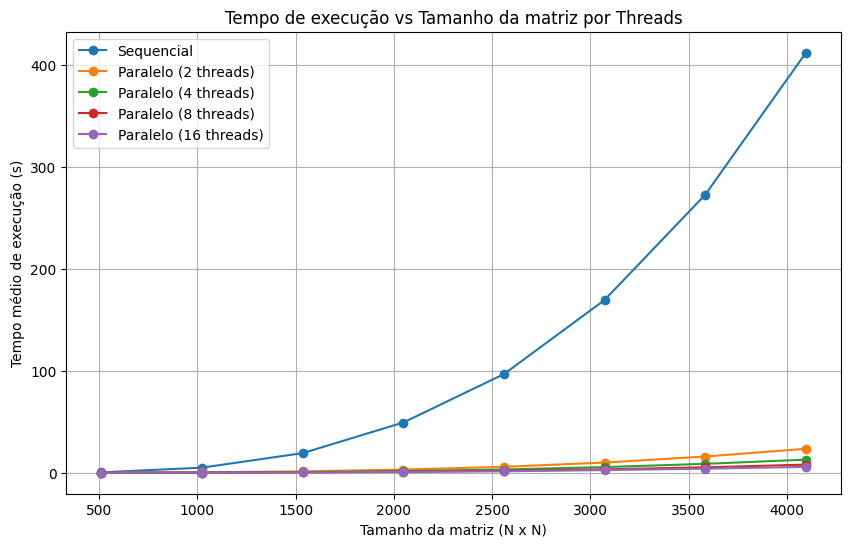
\includegraphics[width=0.8\textwidth]{img/execution-time.png}
		\caption{Tempo de execução (sem otimizações)}
		\label{fig:tempo_execucao}
	\end{figure}

	A Figura \ref{fig:tempo_execucao} mostra o tempo de execução das versões sequencial e paralela
	(sem otimizações) para diferentes tamanhos de matrizes e números de threads. Observa-se que a versão paralela
	tem um desempenho significativamente melhor, especialmente para matrizes maiores e com mais threads. A relação
	entre o tempo de execução e o número de threads é notavel, tendo em vista que quando dobram-se o número de threads,
	o tempo de execução quase reduz pela metade.

	\subsubsection{Speedup}

	\begin{figure}[H]
		\centering
		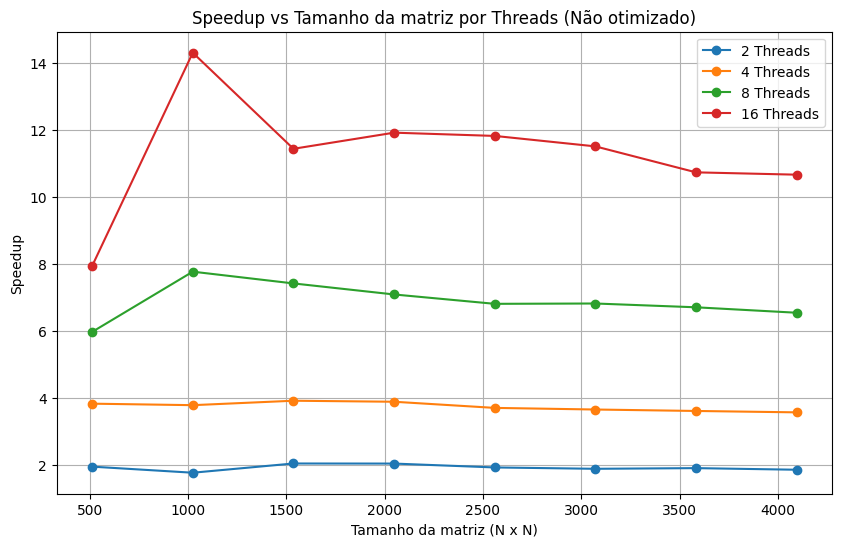
\includegraphics[width=0.8\textwidth]{img/speedup.png}
		\caption{Speedup (sem otimizações)}
		\label{fig:speedup}
	\end{figure}

	A Figura \ref{fig:speedup} apresenta o speedup alcançado pela versão paralela em relação à sequencial para diferentes
	tamanhos de matrizes e números de threads. O speedup se mantém quase constante em relação ao tamanho da matriz, o que
	já era esperado, mas aumenta quase linearmente com o número de threads, indicando uma boa escalabilidade da implementação paralela.

	\subsubsection{Eficiência}

	\begin{figure}[H]
		\centering
		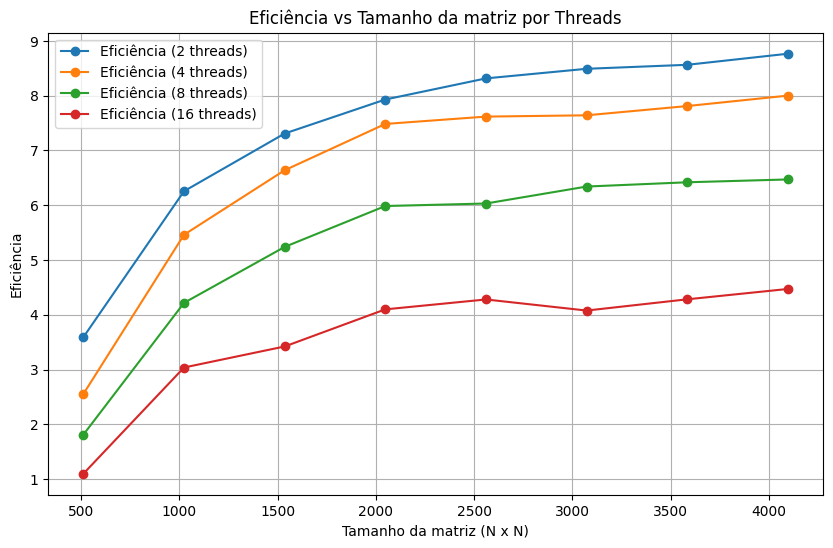
\includegraphics[width=0.8\textwidth]{img/efficiency.png}
		\caption{Eficiência (sem otimizações)}
		\label{fig:eficiencia}
	\end{figure}

	A Figura \ref{fig:eficiencia} mostra a eficiência da versão paralela em relação ao número de threads e tamanhos de matrizes.
	Observa-se que a eficiência diminui com o aumento do número de threads, o que é esperado devido à sobrecarga de gerenciamento de threads. No entanto, a eficiência se mantém relativamente alta (acima de 0.8) para até 8 threads, indicando que a paralelização é eficaz.

	\subsection{Com otimizações}

	Após implementar as otimizações, os testes foram repetidos com a versão paralela otimizada. Foram testados
	os mesmos parametros utilizados anteriormente.

	\subsubsection{Tempo de execução}

	\begin{figure}[H]
		\centering
		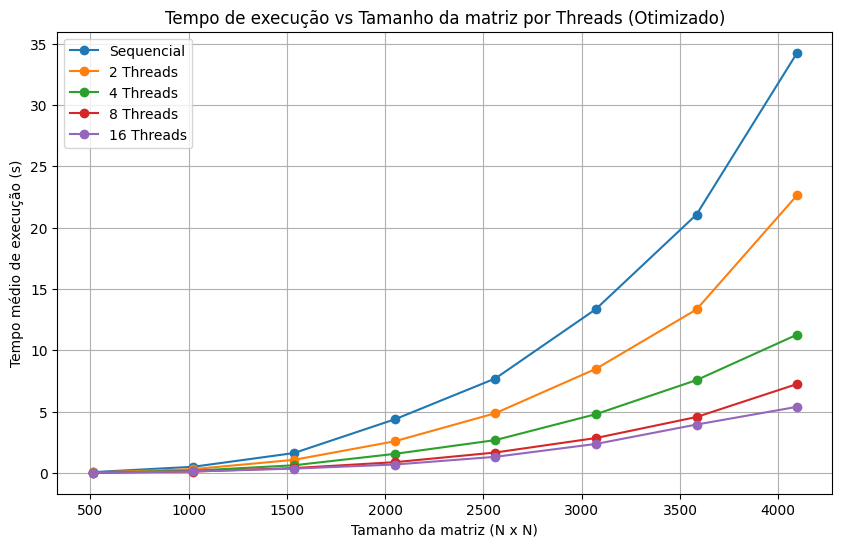
\includegraphics[width=0.8\textwidth]{img/execution-time-opt.png}
		\caption{Tempo de execução (com otimizações)}
		\label{fig:tempo_execucao_otimizado}
	\end{figure}

	É possível observar na Figura \ref{fig:tempo_execucao_otimizado} que o tempo de execução da versão otimizada é
	significativamente menor do que o da versão sem otimizações, especialmente para matrizes maiores. 
	Fazendo com que o tempo de execução caia de mais de 400 segundos para menos de 35 segundos no o pior caso
	em ambas as versões. O tempo de execução diminui ainda mais com o aumento do número de threads, chegando até
	a cerca de 5 segundos para 16 threads em seu pior caso.

	\subsubsection{Speedup}

	\begin{figure}[H]
		\centering
		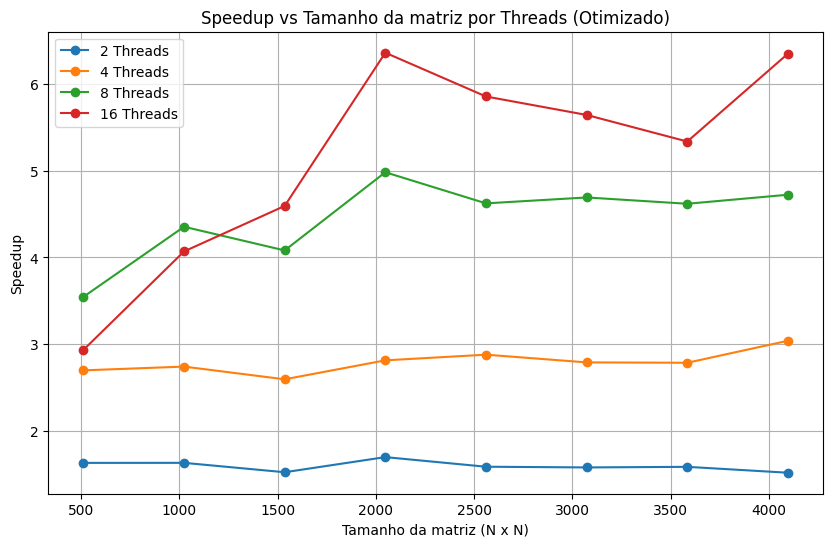
\includegraphics[width=0.8\textwidth]{img/speedup-opt.png}
		\caption{Speedup (com otimizações)}
		\label{fig:speedup_otimizado}
	\end{figure}

	Na Figura \ref{fig:speedup_otimizado}, o speedup da versão otimizada é visivelmente menor em relação à versão sem otimizações.
	Isso se deve ao fato de que a versão sequencial otimizada também teve uma melhora significativa, reduzindo o ganho relativo da versão paralela.
	No entanto, o speedup ainda aumenta com o número de threads, indicando que a paralelização continua sendo eficaz.

	\subsubsection{Eficiência}

	\begin{figure}[H]
		\centering
		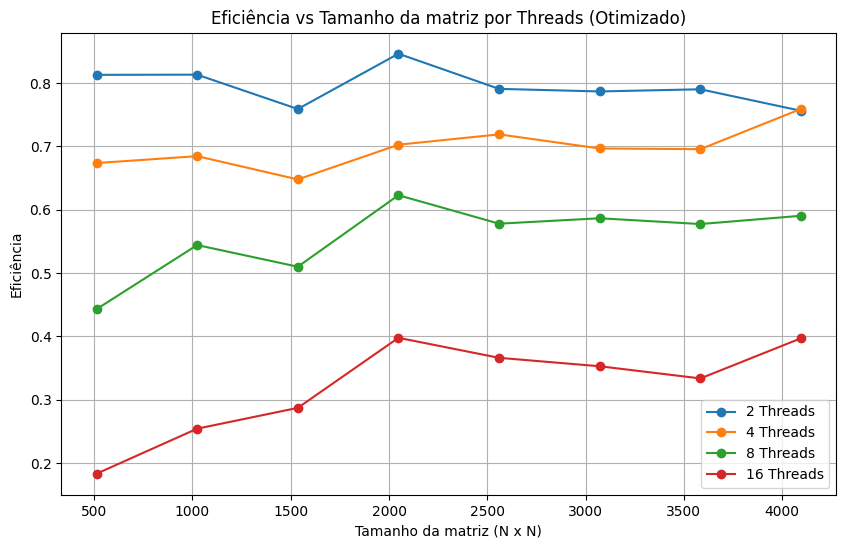
\includegraphics[width=0.8\textwidth]{img/efficiency-opt.png}
		\caption{Eficiência (com otimizações)}
		\label{fig:eficiencia_otimizado}
	\end{figure}

	A Figura \ref{fig:eficiencia_otimizado} mostra que a eficiência da versão otimizada também possui uma eficiência menor em relação à versão sem otimizações.
	Isso é esperado, pois o speedup diminuiu. No entanto, a eficiência se mantém acima de 0.5 para até 8 threads, o que ainda é um resultado positivo, considerando as otimizações aplicadas.

	\section{Discussão}

	\subsection{Comparação entre as versões sequencial e paralela}
	% Análise comparativa dos resultados

	\subsection{Impacto do aumento do número de threads}
	% Como o número de threads afetou o desempenho

	\subsection{Discussão de gargalos e limitações encontradas}
	% Identificar problemas e limitações

	\subsection{Sugestões de melhorias}
	% Propostas para melhorar o desempenho

	\section{Conclusão}

	\subsection{Principais aprendizados do projeto}
	% O que foi aprendido com o projeto

	\subsection{Considerações sobre desempenho obtido}
	% Avaliação geral dos resultados

	\begin{thebibliography}{9}
		\bibitem{latexcompanion} \textit{Orellana, E.}, \texttt{Materiais de slides vistos em aula}

		\bibitem{latexcompanion} \textit{OPENMP}, Disponível em: \texttt{https://www.openmp.org/wp-content/uploads/OpenMP-RefGuide-6.0-OMP60SC24-web.pdf}. Acesso em: 22 de Setembro de 2025.

		\bibitem{knuthwebsite} Brasil Escola, Disponível em: \texttt{https://brasilescola.uol.com.br/matematica/multiplicacao-matrizes.htm}. Acesso em: 22 de Setembro de 2025.

		\bibitem{knuthwebsite} VSP-BERLIN, Disponível em: \texttt{https://svn.vsp.tu-berlin.de/repos/public-svn/publications/kn-old/strc/html/node9.html}. Acesso em: 23 de Setembro de 2025.

		\bibitem{knuthwebsite} Wikipedia, Disponível em: \texttt{https://en.wikipedia.org/wiki/Loop\_nest\_optimization}. Acesso em: 23 de Setembro de 2025.
	\end{thebibliography}
\end{document}